\documentclass[dvipdfmx,12pt]{beamer}

\usepackage{bxdpx-beamer}
\usepackage{pxjahyper}
\usepackage{minijs}
\usetheme{Annarbor}
\usepackage{mathpazo}
\usepackage{amsmath,amssymb}
\usepackage{graphicx}
\usepackage{array}
\usepackage{dcolumn}

\title{Reference Point \\ for the Baseball Players}
\subtitle{Economic evaluation of the behavior of athletes}
\author{Reio TANJI}
\date{June.28,2018}
\institute{Osaka University}

\begin{document}
\begin{frame}
\titlepage
\end{frame}

\section{Introduction}
\begin{frame}\frametitle{Motivation}

 \begin{itemize}
 
 \item To make an economic explanation about the behavior of the athletes, with attention to how the firms : team owners evaluates their performance.
 
 \item In this study, I pick up those of baseball
 
 : Ample observable statistics indicating performance of the players, that are examined their efficiency w.r.t. making earn more scores, or wins.
 
 \end{itemize}

\end{frame}

\begin{frame}\frametitle{References}
 
 \begin{itemize}
  
  \item Pope \& Simonsohn (2011,Association for Phychological Science)
   
  ``Round Numbers as Goals : Evidence From Baseball, SAT Takers, and the Lab''
   
  \item Hakes \& Sauer (2006, Jornal of Economic Perspectives)
   
  ``An Economic Evaluation of the \textit{Moneyball} Hypothesis''
   
  \end{itemize}
 
\end{frame}

\section{Pope \& Simonsohn}
\begin{frame}\frametitle{Pope \& Simonsohn (2011)}

\begin{itemize}

\item Verify that \textbf{round numbers} in performance scales act as \textbf{reference points}, by examing three practical studies.

\item In the first study, they found that baseball players in MLB prefer finising the season with a batting average(AVG) just above .300, to that with just below .300.

\item Data : MLB player's play-by-play data from 1975 to 2008.

Players with at least 200 at bat (打数) : N=8,817

\end{itemize}

\end{frame}

\begin{frame}
\begin{center}

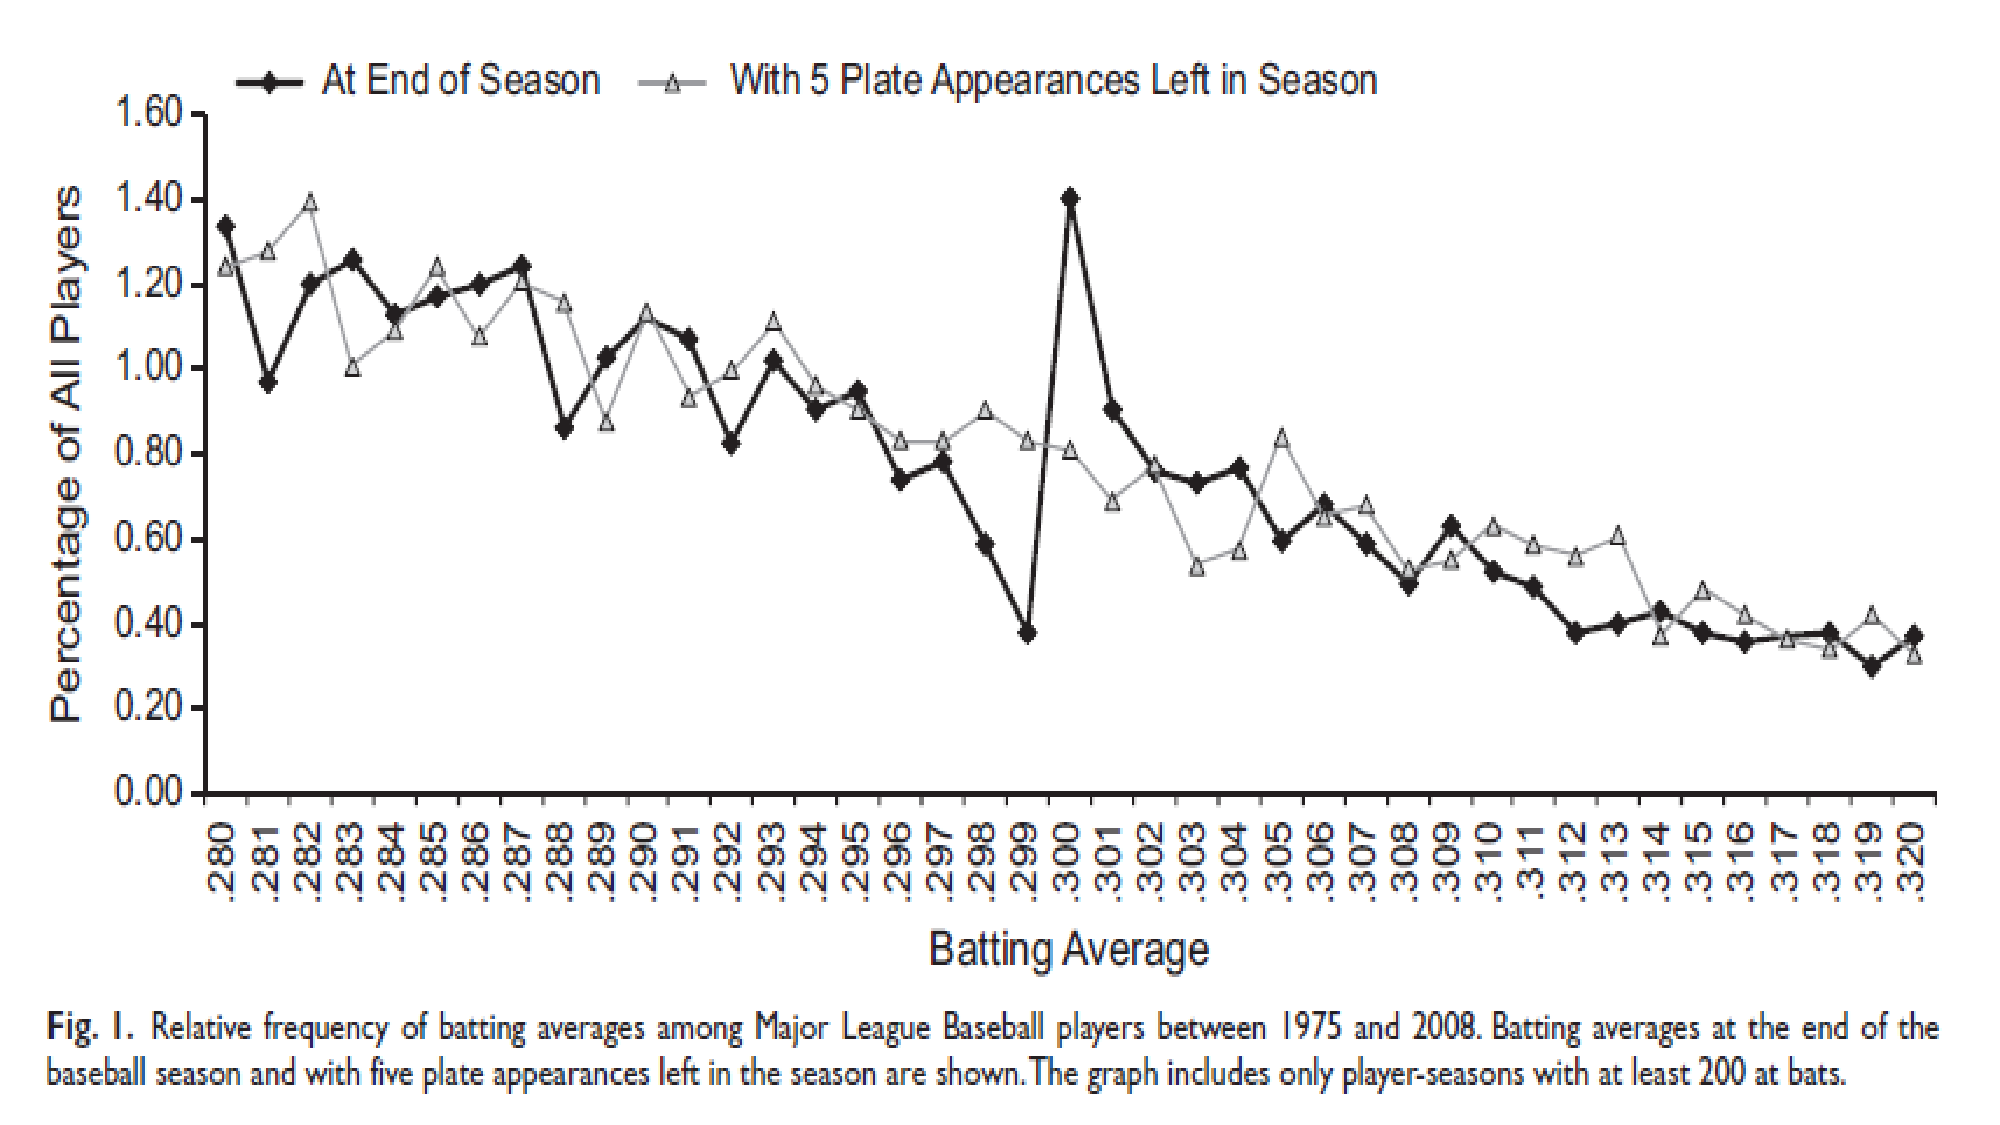
\includegraphics[width=12cm,height=5.25cm]{Pope_Simonsohn_F1.pdf}

\end{center}

 \begin{itemize}
 
 \item Players with .298 or .299 (0.97 \%) $<$ with .300 or .301 (2.30 \%), $Z=7.35$, $p<.001$.
 
 \item Control distribution : when 5 plate appearances left in the season.
 

 \end{itemize}

\end{frame}

\begin{frame}

\begin{center}

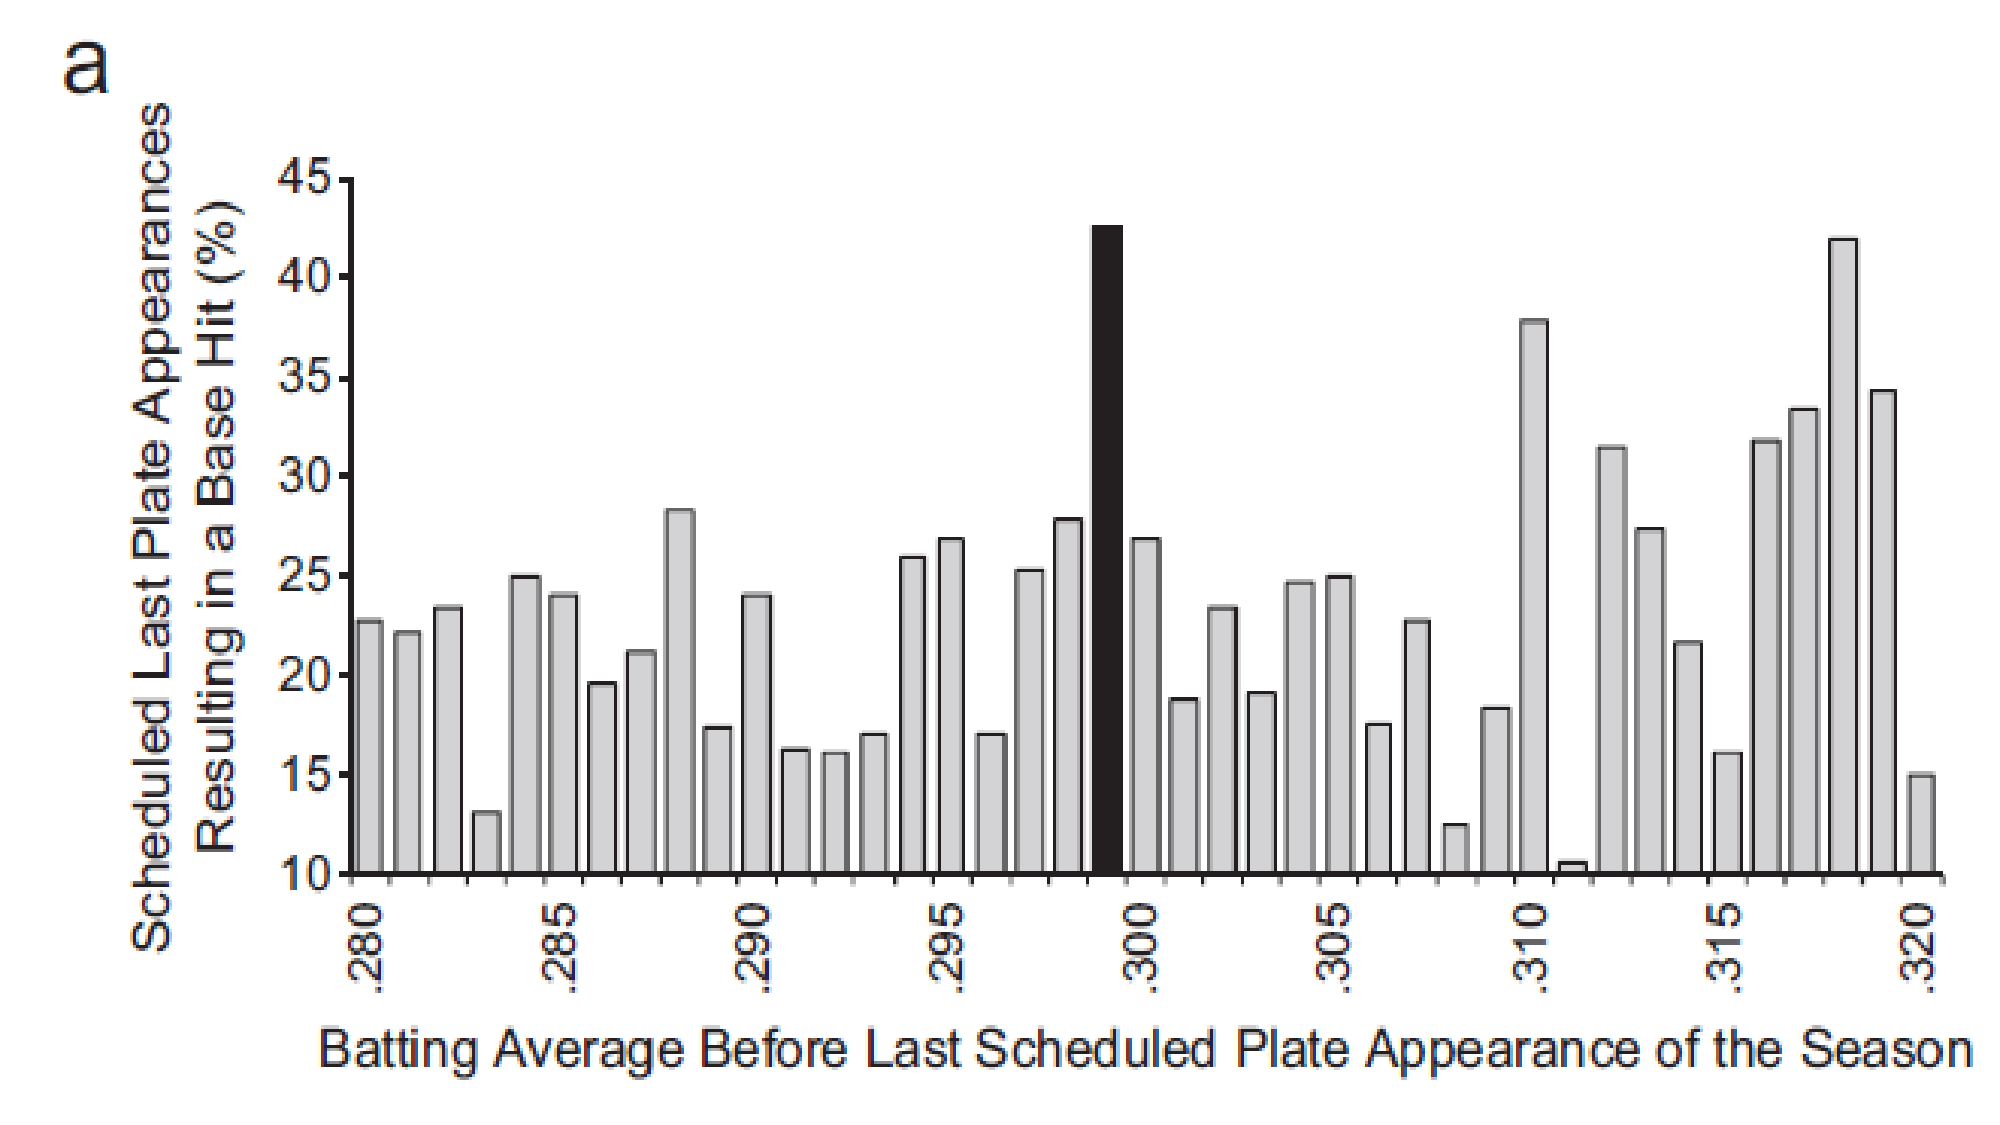
\includegraphics[width=10cm,height=5.75cm]{Pope_Simonsohn_F2A.pdf}

\end{center}

 \begin{itemize}
 
 \item Players with AVG of .299 was likely to get a base hit(43\%) than overall(22.8\%) at their last PA.
 
 $Z=3.62 , p <.001$.
 
 \end{itemize}

\end{frame}

\begin{frame}

\begin{center}

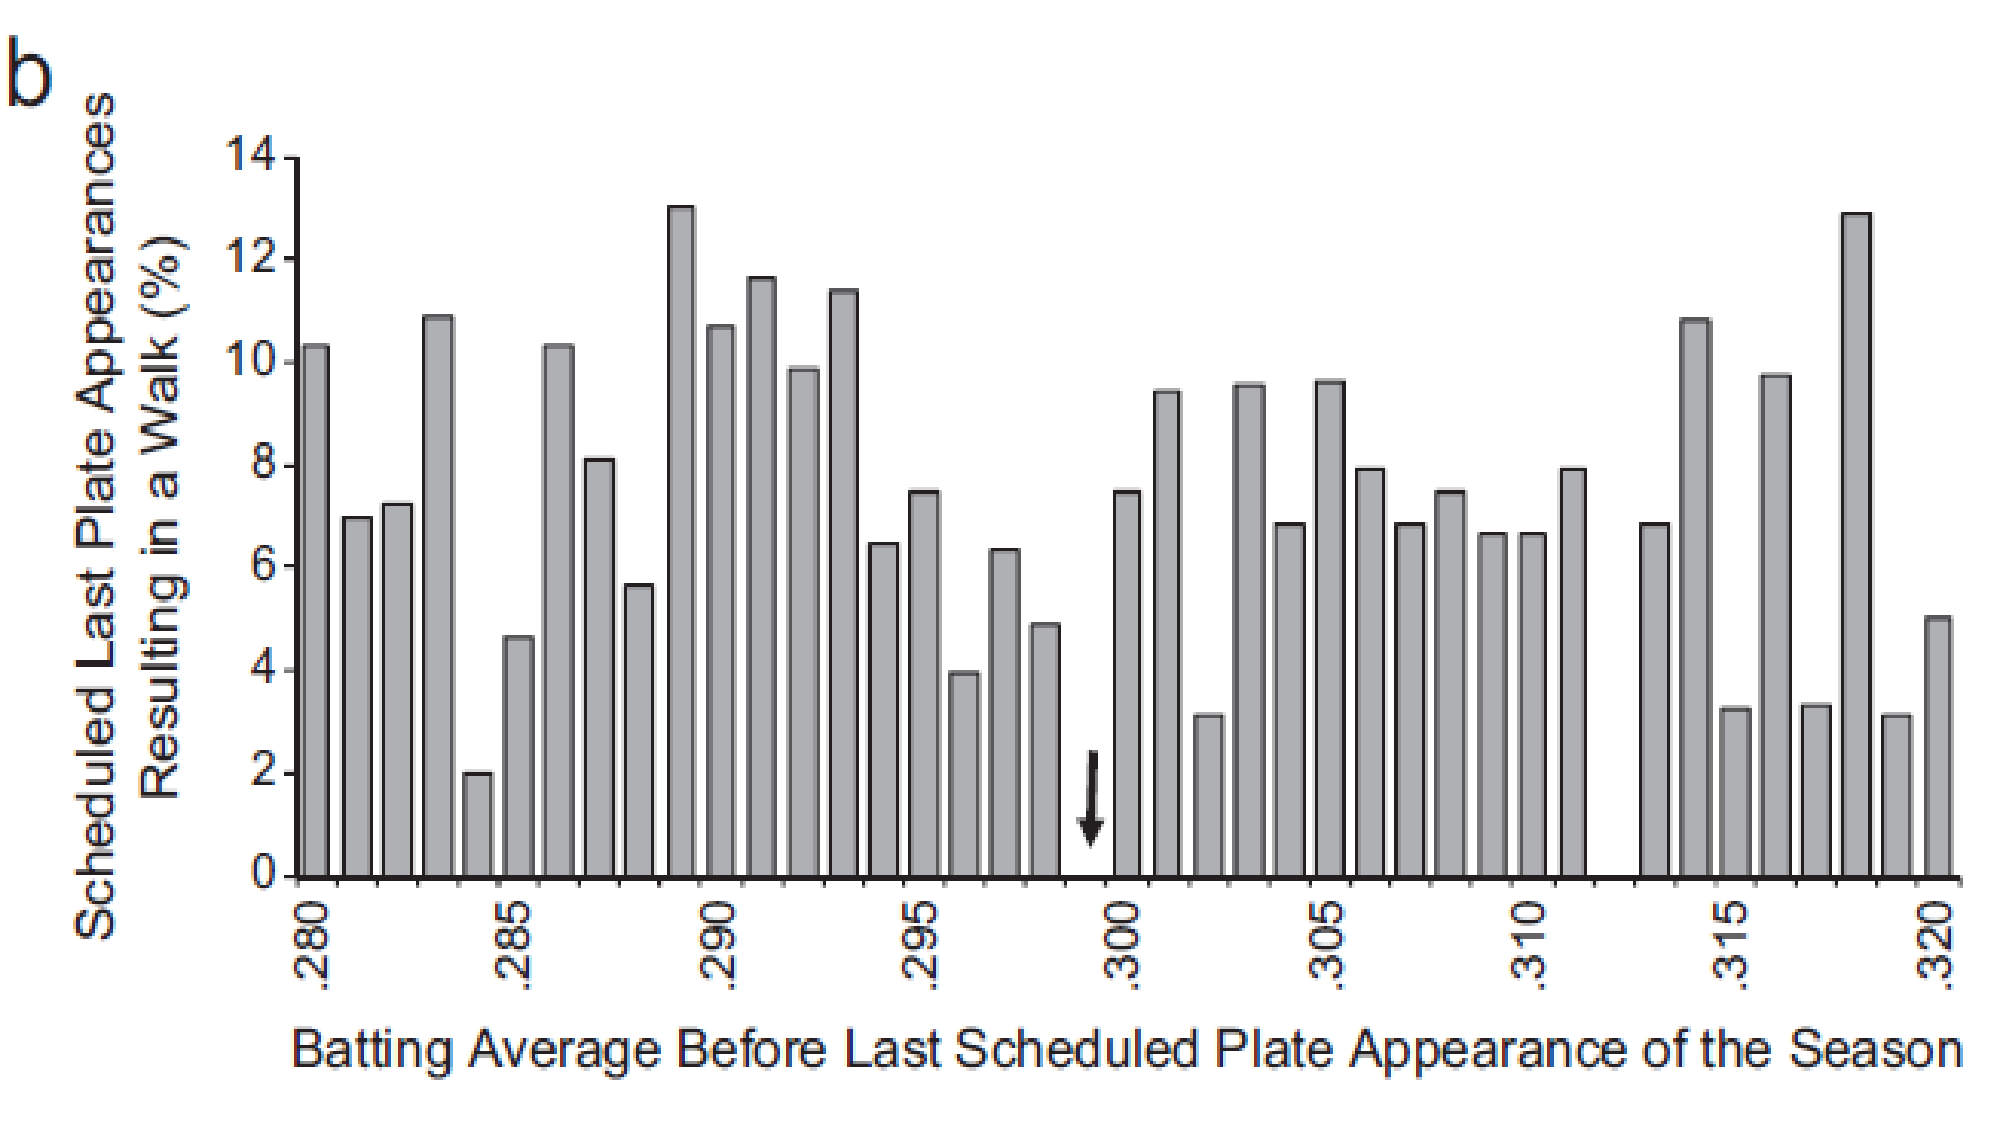
\includegraphics[width=10cm,height=5.75cm]{Pope_Simonsohn_F2B.pdf}

\end{center}

 \begin{itemize}
 
 \item .298 or .299 players tend to walk (四球) than .300 or .301 players.
 
 $Z=2.14$, $p=.032$.
 
 \end{itemize}

\end{frame}

\begin{frame}

\begin{center}

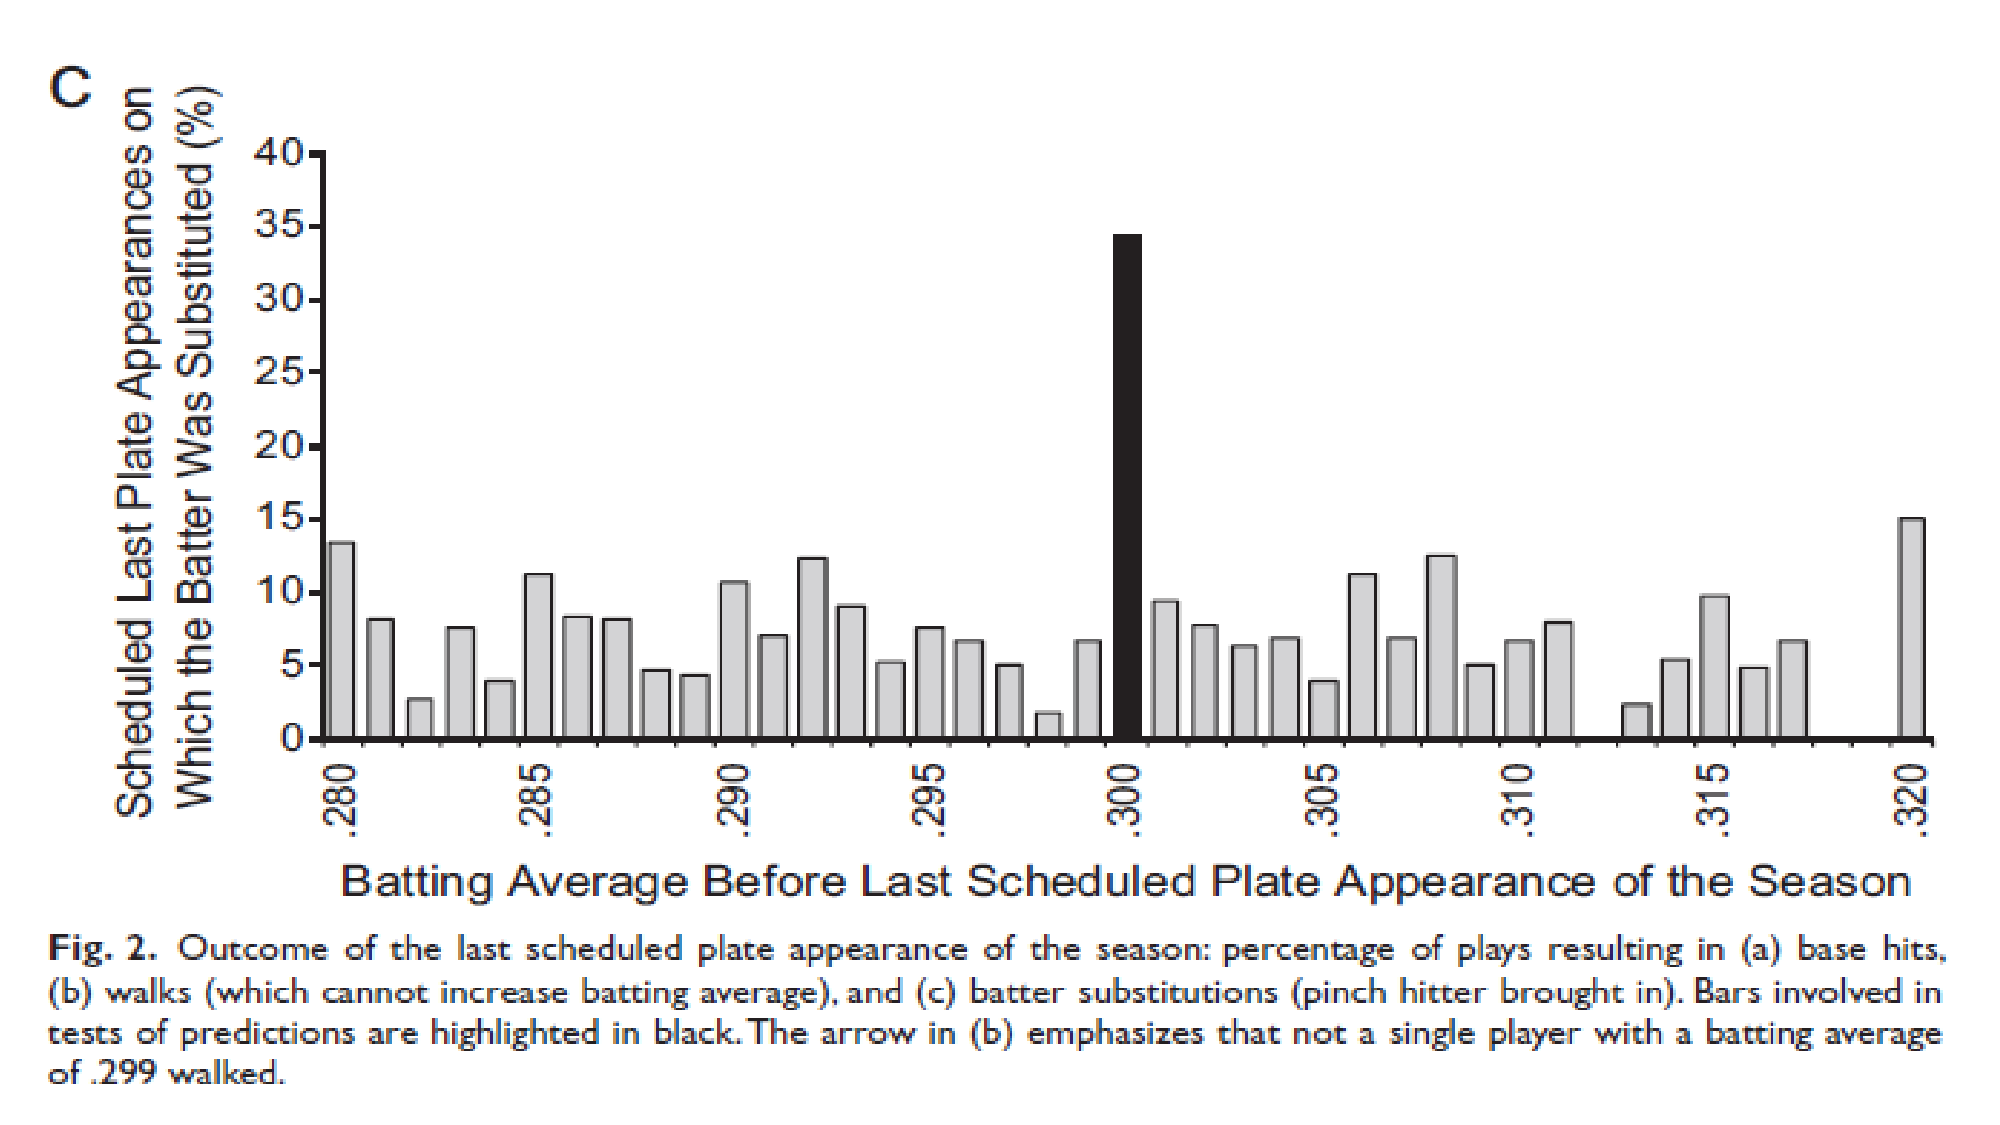
\includegraphics[width=9cm,height=5.75cm]{Pope_Simonsohn_F2C.pdf}

\end{center}

 \begin{itemize}
 
 \item If his AVG is just above .300, then he might end the season earlier by being substituted.
 
 $Z=8.29$ and $p<.001$.
 
 \end{itemize}

\end{frame}

\begin{frame}\frametitle{Pope \& Simonsohn}

 \begin{itemize}
 
 \item The behavior of baseball players proved the existence of the reference point of round numbers, such as batting average of .300.
 
 \item Limitations:
 
 There were only one relevant round number.
 
 Action to improve their performance took place on the last plate appearance.
 
 \end{itemize}

\end{frame}


\section{Hakes \& Sauer}
\begin{frame}\frametitle{Hakes \& Sauer(2006)}

 \begin{itemize}
 \item \textit{``Moneyball Hypothesis''}
 
 : Michael Lewis's claim that the valuation of skills in MLB player's market was grossly inefficient.
 
 \item Members of the Society for American Baseball Research (In short, SABR) have studied that
 on-base percentage (OBP) plays more important role to consider the winning average than batting average, or slugging average.
 
 \item After the publication of ``Moneyball,'' OBP got regarded of more importance than before 
 
 : Players with high batting averages or many homeruns are overestimated.
 
 \end{itemize}

\end{frame}

\begin{frame}\frametitle{Definition}

\begin{align*}
\text{AVG} &= \dfrac{\text{base-hits}}{\text{at-bats}} \\
\text{OBP} &= \dfrac{\text{base-hits} + \text{walks} + \text{hit-by-pitches}} 
{\text{at-bats} + \text{walks} + \text{hit-by-pitches} + \text{sacrifice-flies}} \\
\text{SLG} &= \dfrac{\text{singles} + 2 \times \text{doubles} + 3 \times \text{triples} + 4 \times \text{HRs}}
{\text{at-bats}}
\end{align*}

\end{frame}

\begin{frame}

\begin{center}

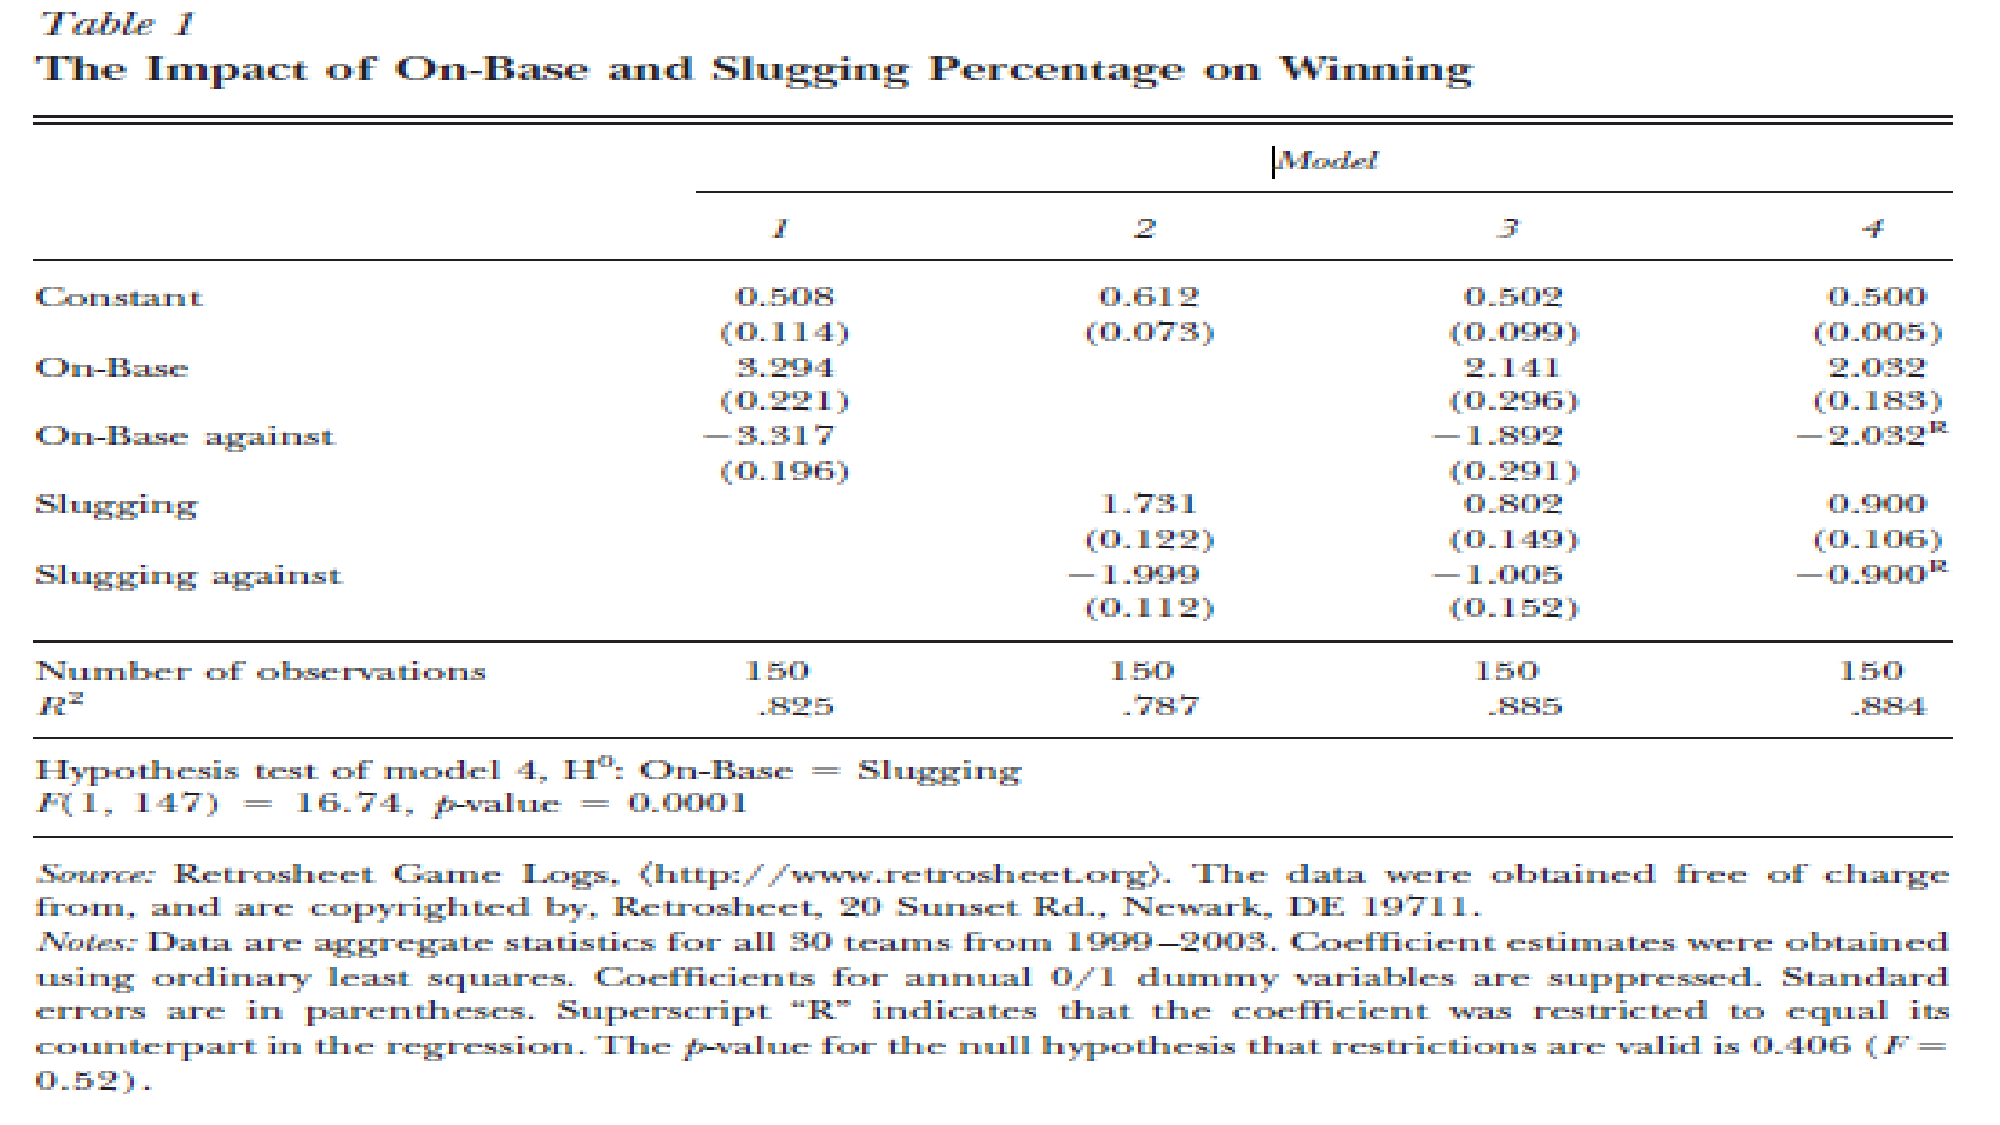
\includegraphics[width=9cm,height=7.75cm]{Hakes_Sauer_T1.pdf}

\end{center}

\end{frame}

\begin{frame}

\begin{center}

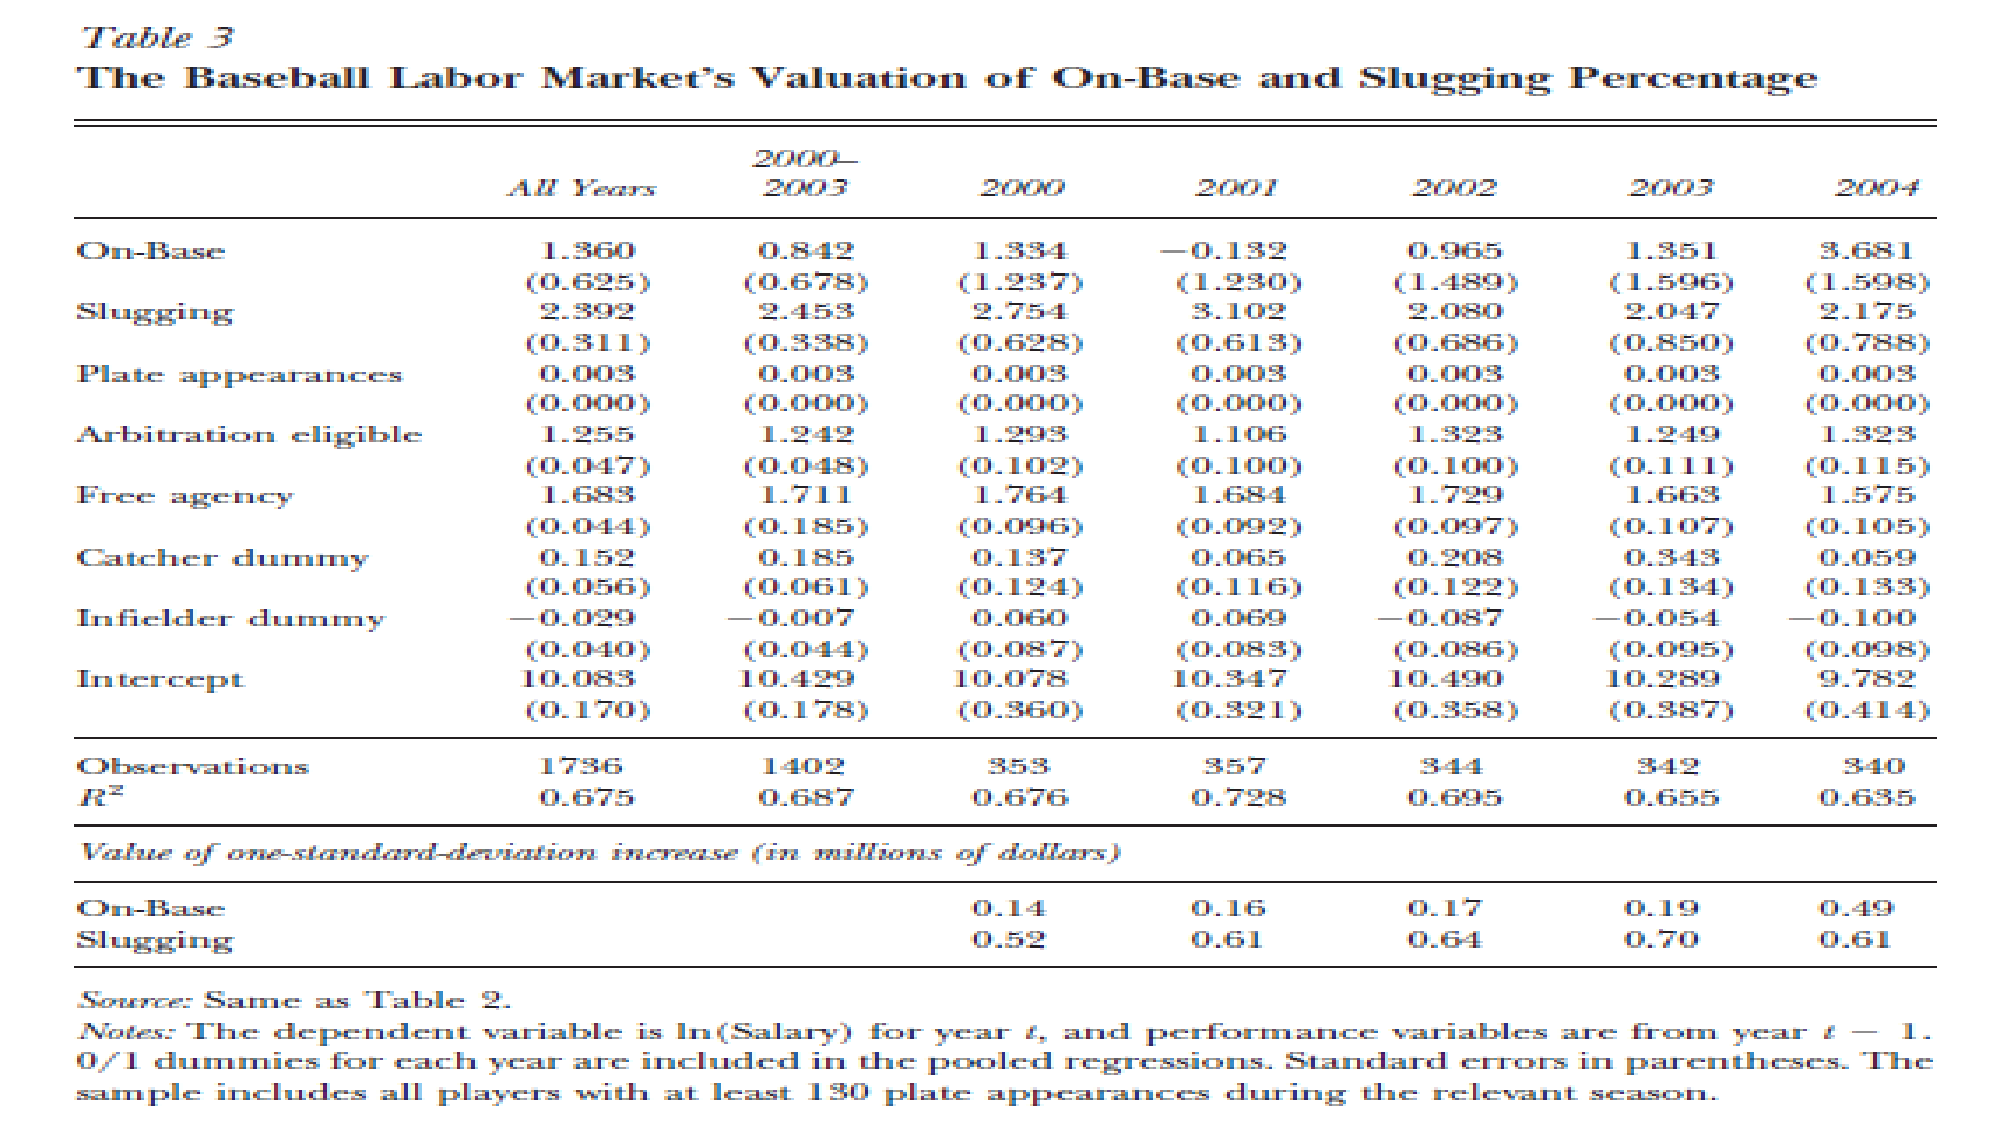
\includegraphics[width=9cm,height=7.75cm]{Hakes_Sauer_T3.pdf}

\end{center}

\end{frame}

\begin{frame}

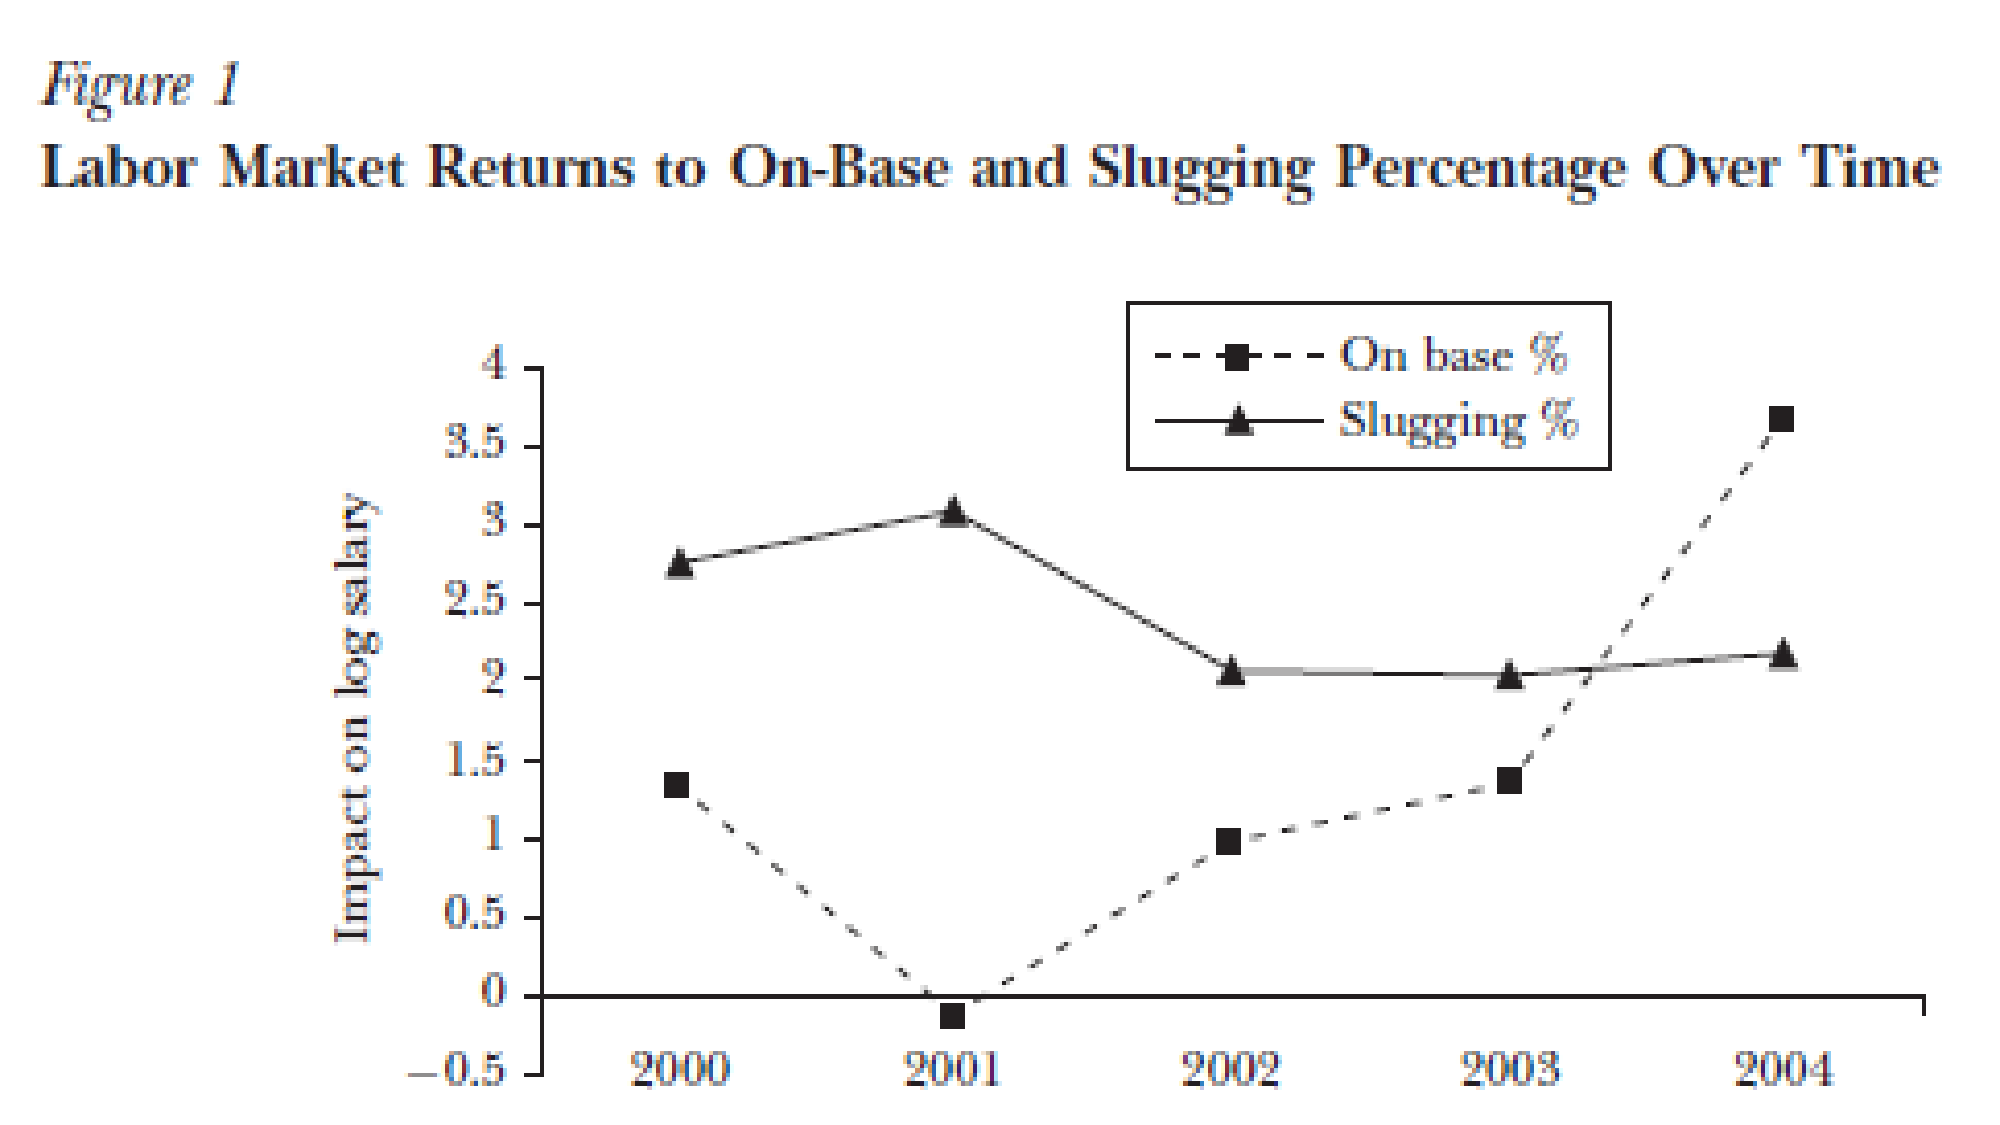
\includegraphics[width=11cm,height=5.75cm]{Hakes_Sauer_F1.pdf}

\end{frame}

\begin{frame}\frametitle{Extension : Reference point of Other Indexes}

 \begin{itemize}
 
 \item On-base percentage may be more important than batting average, when it comes to consider raising winning average, and it reflects players' effort in similar way to batting average.
 
 $\Rightarrow$ Round numbers in on-base percentage may act as reference point, as well as batting-average : .350 or .400.

 \item Moneyball hypothesis emphasized the importance of on-base percentage, rather than batting average : 
 
 After the way to evaluation of the ability revised, players may diminish their effort to meet the reference point, AVG of .300.
 
 \end{itemize}

\end{frame}

\section{Reserch Extension}
\begin{frame}\frametitle{Extension : International Comparision}

 \begin{itemize}
 
 \item In Nippon Professional Baseball (NPB), the contribution of the SABRmetrics is not recognized as much as in MLB :
 
 Evaluation of the players or players' preference may differ from that in MLB.
 
 \item Studies of evaluating performance in MLB
 
 ``Contract Length and the Return to Performance in Major League Baseball'' Krautmann \& Oppenheimer(2002, Journal Of Sports Economics)
 
 ``Analyzing Major League Baseball Player's Performance Based On Age And Experience'' K.Ng(2017,Journal of Sports Economics \& Management)
 
 \end{itemize}

\end{frame}


\begin{frame}\frametitle{Data}

 \begin{itemize}
 
 \item Sortable team stats of Nippon Professional Baseball (NPB), from 2008 to 2017.
 
 : N=120
 
 \item Indexes : Winning average (勝率 : WA), Runs (得点 : R) Runs allowed (失点 : RA)
 , Batting average (AVG), On-base percentage (出塁率 : OBP) Slugging percentage(長打率 : SLG)
 
 \end{itemize}

\end{frame}

\begin{frame}\frametitle{Model}

 \begin{itemize}
 
 \item Confirm that also in NPB, OBP contributes better to the Win Average than AVG or SLG.
 
 Applying OLS,
 
 \[\textit{WA}_i = \beta \mathbf{X}_i + \textit{RA}_i + u_i \]
 
 \[\textit{R}_i = \gamma \mathbf{X}_i + v_i \]
  
  \begin{align*}
  \textit{WA}_i &: \text{Win average of team } i \\
  \textit{R}_i &: \text{Runs of team } i \\
  \mathbf{X}_i &: \text{OBP, SLG and AVG of the team } i
  \end{align*}
 
 \end{itemize}

\end{frame}

\begin{frame}\frametitle{Results:Winning Averages}

\tiny

% Table created by stargazer v.5.2.2 by Marek Hlavac, Harvard University. E-mail: hlavac at fas.harvard.edu
% Date and time: 火, 6 26, 2018 - 19:48:30
% Requires LaTeX packages: dcolumn 
\begin{table}[!htbp] \centering 
  \caption{Contribution to winning averages} 
  \label{} 
\begin{tabular}{@{\extracolsep{5pt}}lD{.}{.}{-3} D{.}{.}{-3} } 
\\[-1.8ex]\hline 
\hline \\[-1.8ex] 
 & \multicolumn{2}{c}{\textit{Dependent variable:}} \\ 
\cline{2-3} 
\\[-1.8ex] & \multicolumn{2}{c}{WA} \\ 
\\[-1.8ex] & \multicolumn{1}{c}{(1)} & \multicolumn{1}{c}{(2)}\\ 
\hline \\[-1.8ex] 
 OBP & 1.448^{***} &  \\ 
  & (0.316) &  \\ 
  AVG &  & 1.194^{***} \\ 
  &  & (0.425) \\ 
  SLG & 1.257^{***} & 1.369^{***} \\ 
  & (0.146) & (0.170) \\ 
  RA & -0.001^{***} & -0.001^{***} \\ 
  & (0.00004) & (0.00004) \\ 
  Constant & -0.024 & 0.100 \\ 
  & (0.074) & (0.072) \\ 
 \hline \\[-1.8ex] 
Observations & \multicolumn{1}{c}{120} & \multicolumn{1}{c}{120} \\ 
R$^{2}$ & \multicolumn{1}{c}{0.825} & \multicolumn{1}{c}{0.807} \\ 
Adjusted R$^{2}$ & \multicolumn{1}{c}{0.821} & \multicolumn{1}{c}{0.802} \\ 
Residual Std. Error (df = 116) & \multicolumn{1}{c}{0.031} & \multicolumn{1}{c}{0.032} \\ 
F Statistic (df = 3; 116) & \multicolumn{1}{c}{182.732$^{***}$} & \multicolumn{1}{c}{161.505$^{***}$} \\ 
\hline 
\hline \\[-1.8ex] 
\textit{Note:}  & \multicolumn{2}{r}{$^{*}$p$<$0.1; $^{**}$p$<$0.05; $^{***}$p$<$0.01} \\ 
\end{tabular} 
\end{table} 

\large

\end{frame}
\begin{frame}\frametitle{Results:Runs}

\tiny

% Table created by stargazer v.5.2.2 by Marek Hlavac, Harvard University. E-mail: hlavac at fas.harvard.edu
% Date and time: 火, 6 26, 2018 - 19:48:17
% Requires LaTeX packages: dcolumn 
\begin{table}[!htbp] \centering 
  \caption{Contribution to runs} 
  \label{} 
\begin{tabular}{@{\extracolsep{5pt}}lD{.}{.}{-3} D{.}{.}{-3} } 
\\[-1.8ex]\hline 
\hline \\[-1.8ex] 
 & \multicolumn{2}{c}{\textit{Dependent variable:}} \\ 
\cline{2-3} 
\\[-1.8ex] & \multicolumn{2}{c}{R} \\ 
\\[-1.8ex] & \multicolumn{1}{c}{(1)} & \multicolumn{1}{c}{(2)}\\ 
\hline \\[-1.8ex] 
 OBP & 2,213.855^{***} &  \\ 
  & (225.357) &  \\ 
  AVG &  & 1,786.436^{***} \\ 
  &  & (354.230) \\ 
  SLG & 1,650.727^{***} & 1,818.552^{***} \\ 
  & (99.793) & (137.220) \\ 
  Constant & -774.218^{***} & -583.790^{***} \\ 
  & (51.748) & (58.846) \\ 
 \hline \\[-1.8ex] 
Observations & \multicolumn{1}{c}{120} & \multicolumn{1}{c}{120} \\ 
R$^{2}$ & \multicolumn{1}{c}{0.918} & \multicolumn{1}{c}{0.877} \\ 
Adjusted R$^{2}$ & \multicolumn{1}{c}{0.917} & \multicolumn{1}{c}{0.875} \\ 
Residual Std. Error (df = 117) & \multicolumn{1}{c}{21.897} & \multicolumn{1}{c}{26.809} \\ 
F Statistic (df = 2; 117) & \multicolumn{1}{c}{656.783$^{***}$} & \multicolumn{1}{c}{418.676$^{***}$} \\ 
\hline 
\hline \\[-1.8ex] 
\textit{Note:}  & \multicolumn{2}{r}{$^{*}$p$<$0.1; $^{**}$p$<$0.05; $^{***}$p$<$0.01} \\ 
\end{tabular} 
\end{table} 
 
\large

\end{frame}

\section{Appendix}
\begin{frame}

\begin{center}

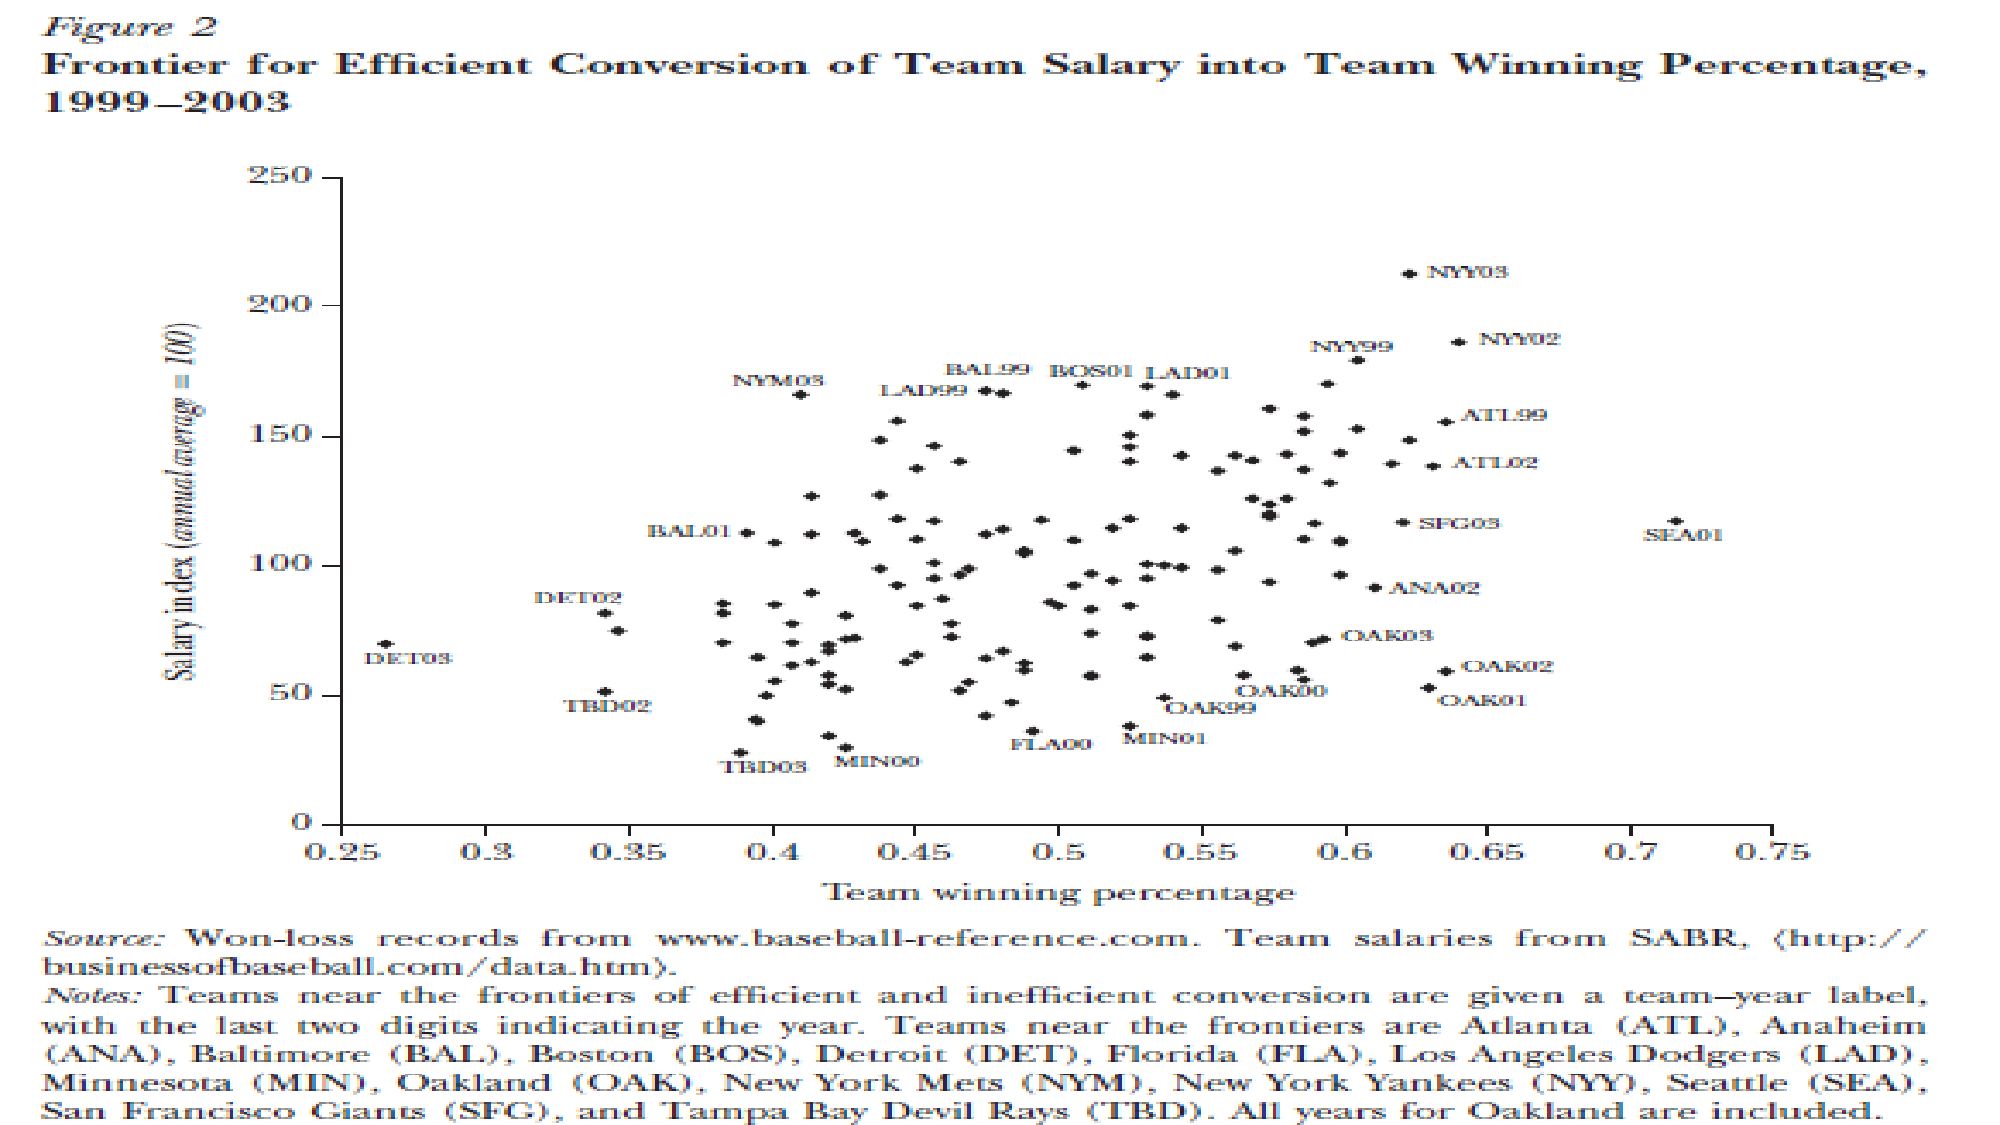
\includegraphics[width=9.5cm,height=8.4cm]{Hakes_Sauer_F2.pdf}

\end{center}

\end{frame}


\end{document}